\documentclass[a4paper,10pt,titlepage,bibtotoc,bibtotocnumbered]{scrreprt}

\usepackage[utf8]{inputenc}
\usepackage[pdftex]{graphicx}
\usepackage{lscape}
\usepackage{rotating}
\usepackage{ulem}


%%%%%%%Here you have to choose german or english texts in your submissions
%German submission
%\usepackage[ngerman]{babel}
%English submission
\usepackage[english]{babel}

%Graphics and pictures
\usepackage[caption=false]{subfig}
\usepackage{float}
\restylefloat{figure}
\usepackage{placeins}

%Enumerations
\usepackage{enumerate}
\usepackage{mdwlist}

%Math symbols
\usepackage{amsmath}
\usepackage{amssymb}

%Coloring of tables
\usepackage{longtable}
\usepackage{xcolor, colortbl}

%Code representation
\usepackage{listings}

%Diagrams with tikZ
\usepackage{tikz}
\usetikzlibrary{shapes.geometric, arrows, positioning}

\newcommand{\students}[1]{\def\vstudents{#1}}
\newcommand{\labtime}[1]{\def\vlabtime{#1}}
\newcommand{\supervisor}[2]{\def\vsupervisor{\href{#2}{#1}}}


\usepackage[marginpar=2cm,
	reversemp,
	includehead,
	includefoot,
	bindingoffset=0cm,
	textheight=23cm,
	hdivide={3.5cm,*,3.5cm},
	vdivide={*,23cm,*}
	]{geometry}


\usepackage[pdftex,	pdfauthor={},
				pdftitle={Cinema Management Application},
				pdfsubject={Lab for Software Engineering WS22/23},
				breaklinks=true,
				colorlinks=true,
				linkcolor=black,
				urlcolor=blue,%blue
				citecolor=red,%red
	        		pdfpagemode=None,
%   			    	pdffitwindow=true,
        			a4paper=true,
				plainpages=false,
				pdfpagelabels,
				pageanchor=false,
				pdfstartpage=1,
           ]{hyperref}

\usepackage{csquotes}

\begin{document}


%-------------------- Declaration part --------------------------------------------
%-------------------- Here you have to add all group members, your lab date -------
%-------------------- and the name of your supervisor -----------------------------
\students{Ifrat Jahan (3098878)\\Jennifer Maxisch (3106694)\\Georgios Adamos (3093306)\\Thomas Klimek (3067855)\\Melvin van der Linde (3106762)}
\labtime{Do. 12-14}
\supervisor{Marcel Schweikert}{marcel.schweikert@stud.uni-due.de}
%----------------------------------------------------------------------------------
%----------------------------------------------------------------------------------



\pagenumbering{roman}

\begin{titlepage}
\centering
\enlargethispage*{40mm}

\vspace*{-10mm}

\begin{minipage}[c]{0.25\textwidth}
\hspace*{-22mm}

\includegraphics[height=45pt]{figures/logo_uni}\linebreak
\end{minipage}
\begin{minipage}[r]{0.74\textwidth}
\vspace*{1mm}
\begin{flushright}
\Large{Lab for Software Engineering}\linebreak
\large{Winter term 2022/2023}\linebreak
\end{flushright}
\end{minipage}
\hspace*{-18mm}

\textcolor{blue}{\rule{154mm}{0.2mm}}


\vspace*{55mm}\vfill

\textit{Lab for Software Engineering}\vspace*{4mm}

\Huge{Cinema Management Application}\vspace*{7mm}

\Large{\vstudents}\vspace*{9mm}


\normalsize{\today}



\vspace*{80mm}

\textcolor{blue}{\rule{\textwidth}{0.2mm}}
\begin{flushleft}
\sf University of Duisburg-Essen $\cdot$ Faculty of Engineering
\large{Working group \href{http://swe.uni-due.de}{Software Engineering} -- Prof. Dr. M. Heisel}\\

\small{Date: \vlabtime- Supervisor: \vsupervisor}
\end{flushleft}

\end{titlepage}


\tableofcontents
\listoffigures

%------------
%------------The structure is the same as used in the lecture.
%------------You can specify new sections included in each chapter and you can also add new subsections.
%------------
%------------
\chapter{Analysis}
\section{A1}

%---------------
%---------------The style of enumerations is already given (e.g. R1, R2,...)
%---------------Just add \item before each element
%---------------
%---------------
\subsection{Requirements \& Domain-Knowledge}

\subsubsection{Requirements}
\begin{enumerate}[R1]
	\item\label{enum:R1} Customers can create an account by providing an e-mail address and a password. If an e-mail address which is already associated with an account is provided, account creation fails.
    \item Customers can log in by providing their e-mail address and their password.
    \item A logged in customer can log out.
    \item\label{enum:R4} A customer can browse available showings, ascendingly sorted by date.
    \item\label{enum:R5} A logged in customer can book tickets by selecting the showing from the browsing list and selecting the desired seats. A showing can only be booked up to 15 minutes before it starts.
    \item Staff can add new showings to the database by providing the required data.
    \item\label{enum:R7} Once a showing starts it is marked as \enquote{archived}.
    \item\label{enum:R8} Archived showings are visible to staff, but not to customers.
    \item Staff can cancel showings. When a show is cancelled all customers who booked tickets for it are notified via e-mail and the showing is then deleted.
    \item Showings which took place a year ago or longer are automatically removed from the database.
    \item When a showing is deleted its associated bookings are also deleted.

\end{enumerate}

\subsubsection{Facts}
\begin{enumerate}[F1]
	\item A showing consists of the title of the movie, its duration, the date date, the hall number and unique ID.
	\item A hall consists of a number of rows, a number of seats per row and a unique hall number.
    \item Only one person at a time can sit in a seat.
\end{enumerate}

\subsubsection{Assumptions}
\begin{enumerate}[{A}1]
	\item A web application is a good choice for implementing the desired functionality and all customers are able to use it.
	\item Customers only provide e-mail addresses they can access.
    \item Customers will stay up to date with the list of available showings.
    \item Every booking is paid via an external service.
    \item Staff will only add showings which take place in the future.
\end{enumerate}

%---------------
%---------------You can use the following code snippet to inclue pictures into your document.
%---------------\caption command places a little description under the picture.
%---------------\label is used to reference the picture in the text with command \ref{figure:contextDiagram}.
%---------------
\subsection{Contextdiagram}
\begin{figure}[H]
	\centering
  	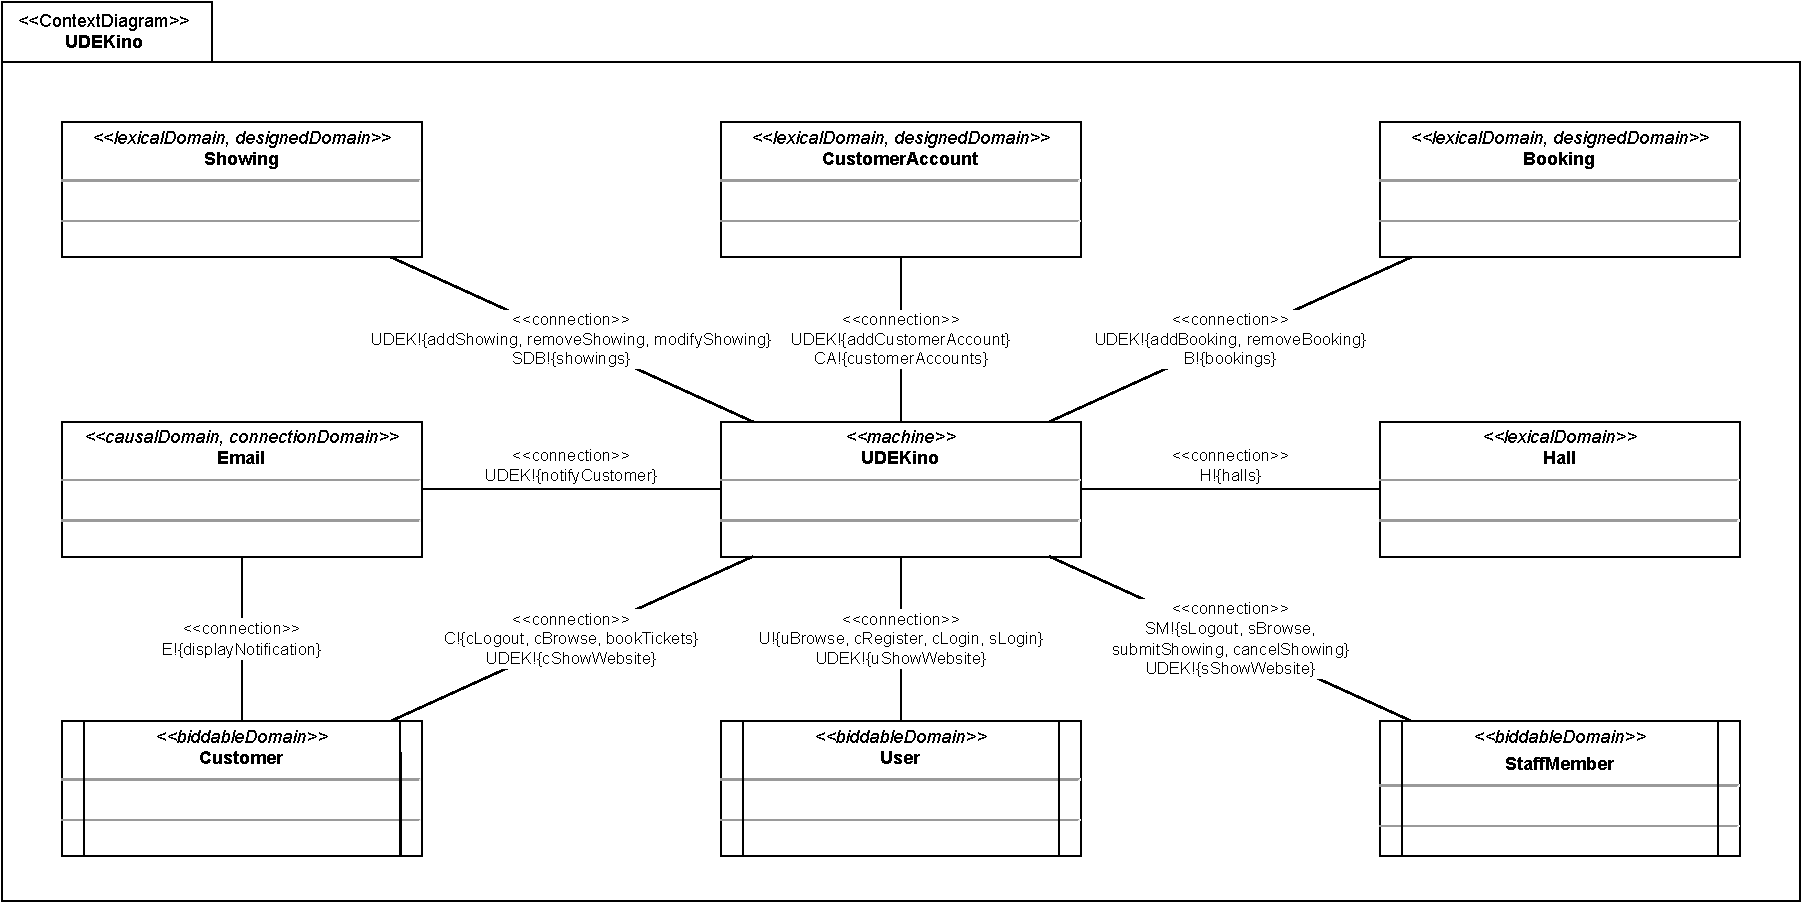
\includegraphics[width=0.9\textwidth]{figures/02/a02_context_diagram.pdf}
	\caption{Contextdiagram}
	\label{figure:contextDiagram}
\end{figure}


\newpage\section{A2}
We can derive the following problem diagrams

\begin{figure}[H]
    \centering
    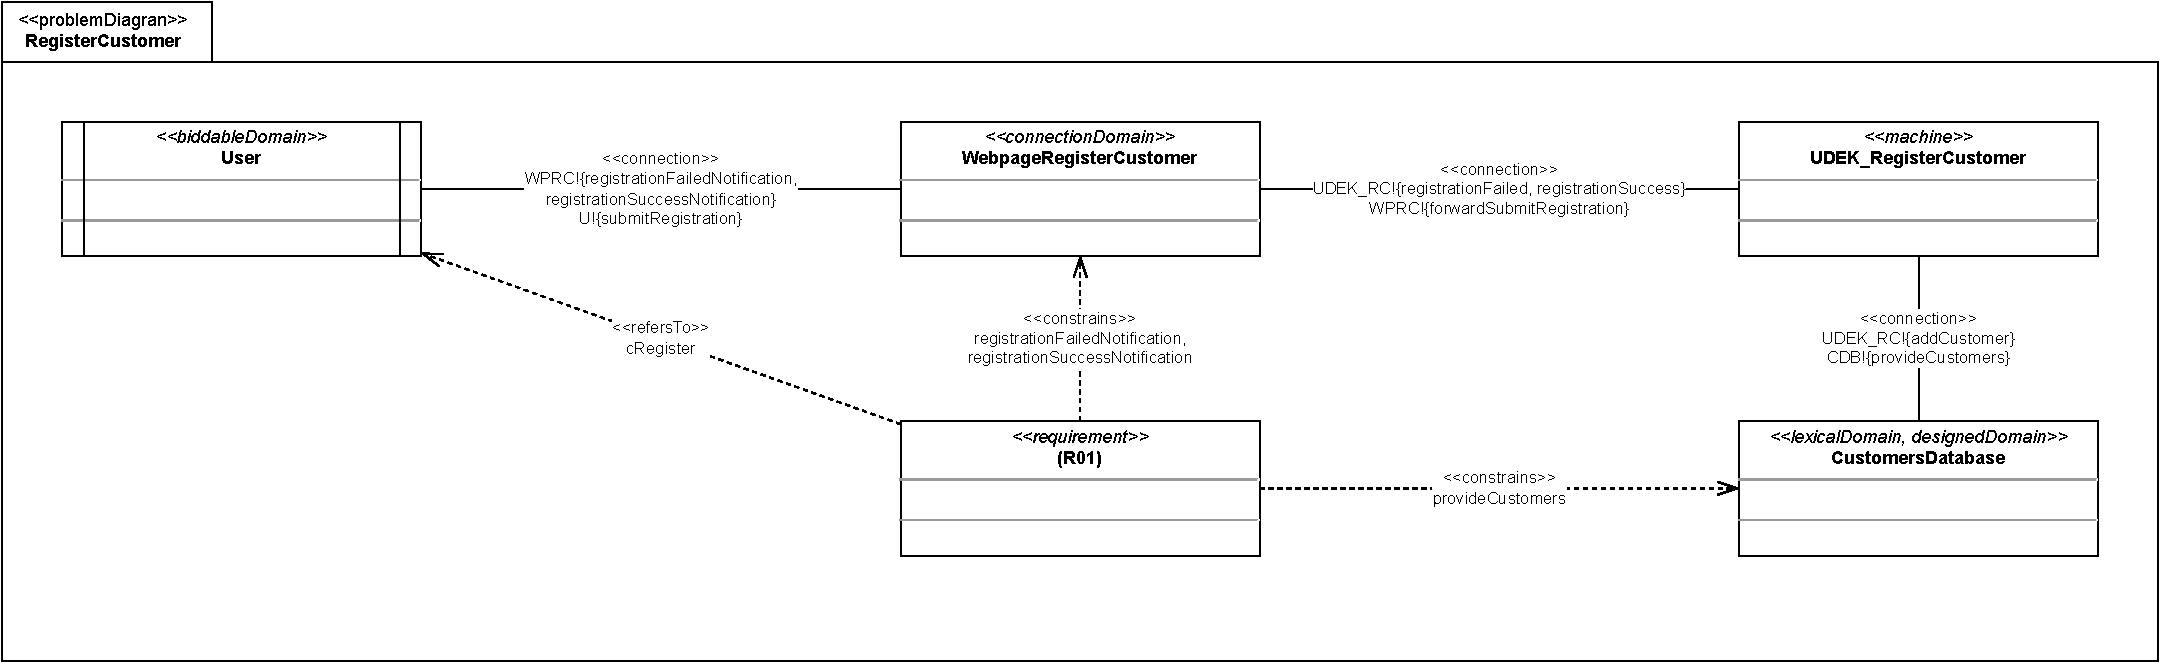
\includegraphics[width=0.9\textwidth]{figures/03/a03_problem_diagram_1-PD.pdf}
    \caption{Problem diagram for R\ref{enum:R1}}
    \label{figure:pdR1}
\end{figure}

\begin{figure}[H]
    \centering
    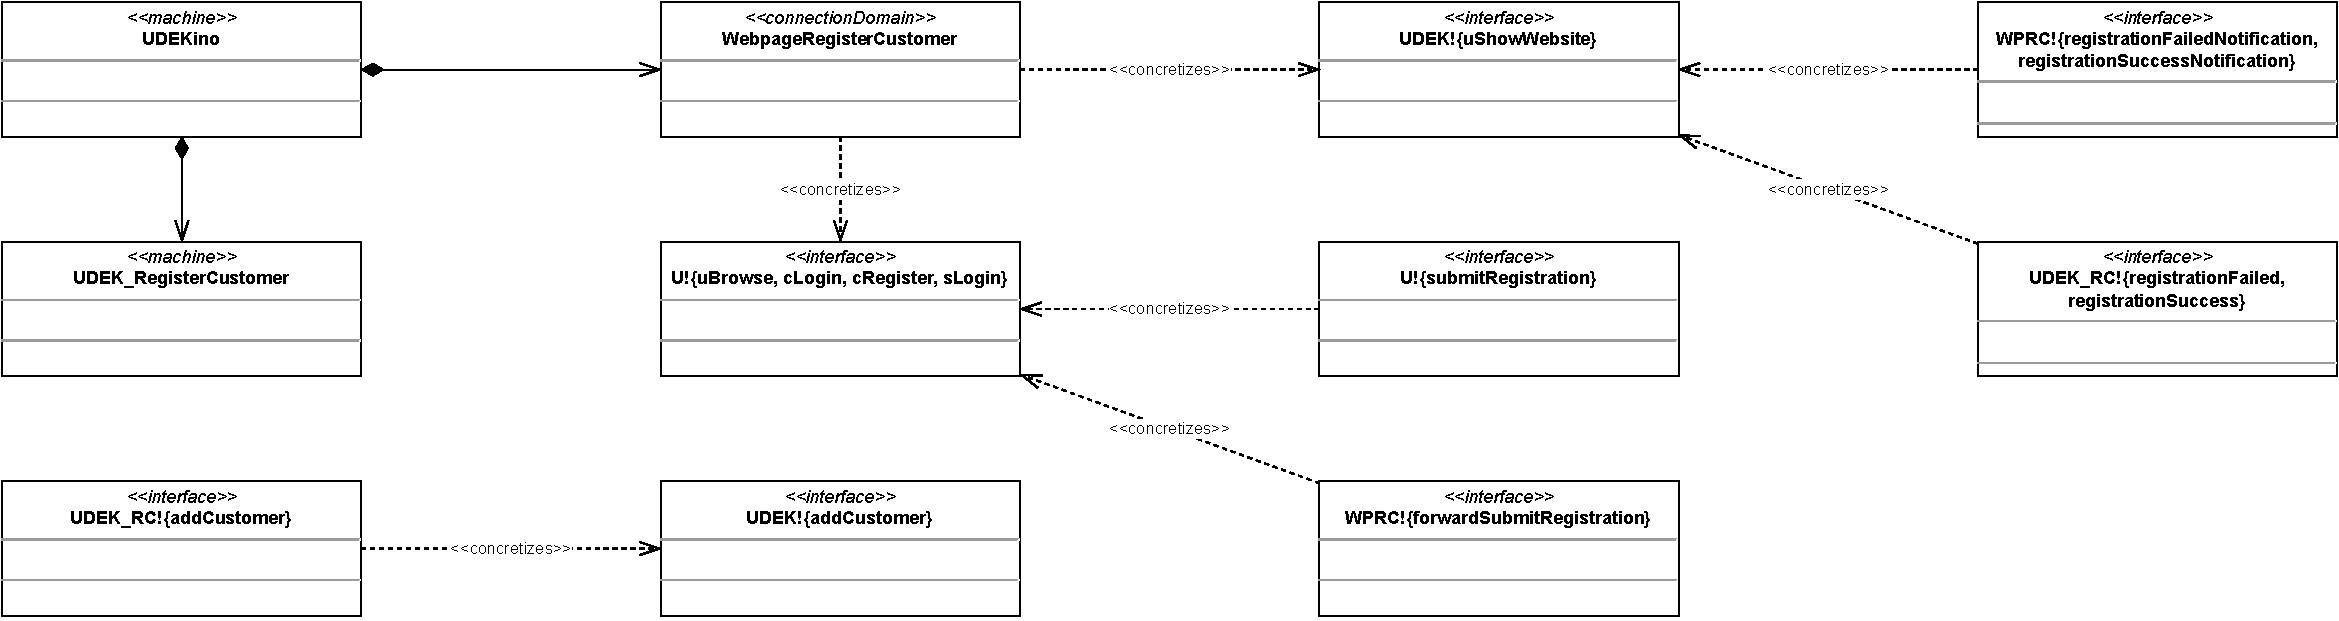
\includegraphics[width=0.9\textwidth]{figures/03/a03_problem_diagram_1-Mapping.pdf}
    \caption{Mapping diagram for R\ref{enum:R1}}
    \label{figure:mdR1}
\end{figure}

\begin{figure}[H]
    \centering
    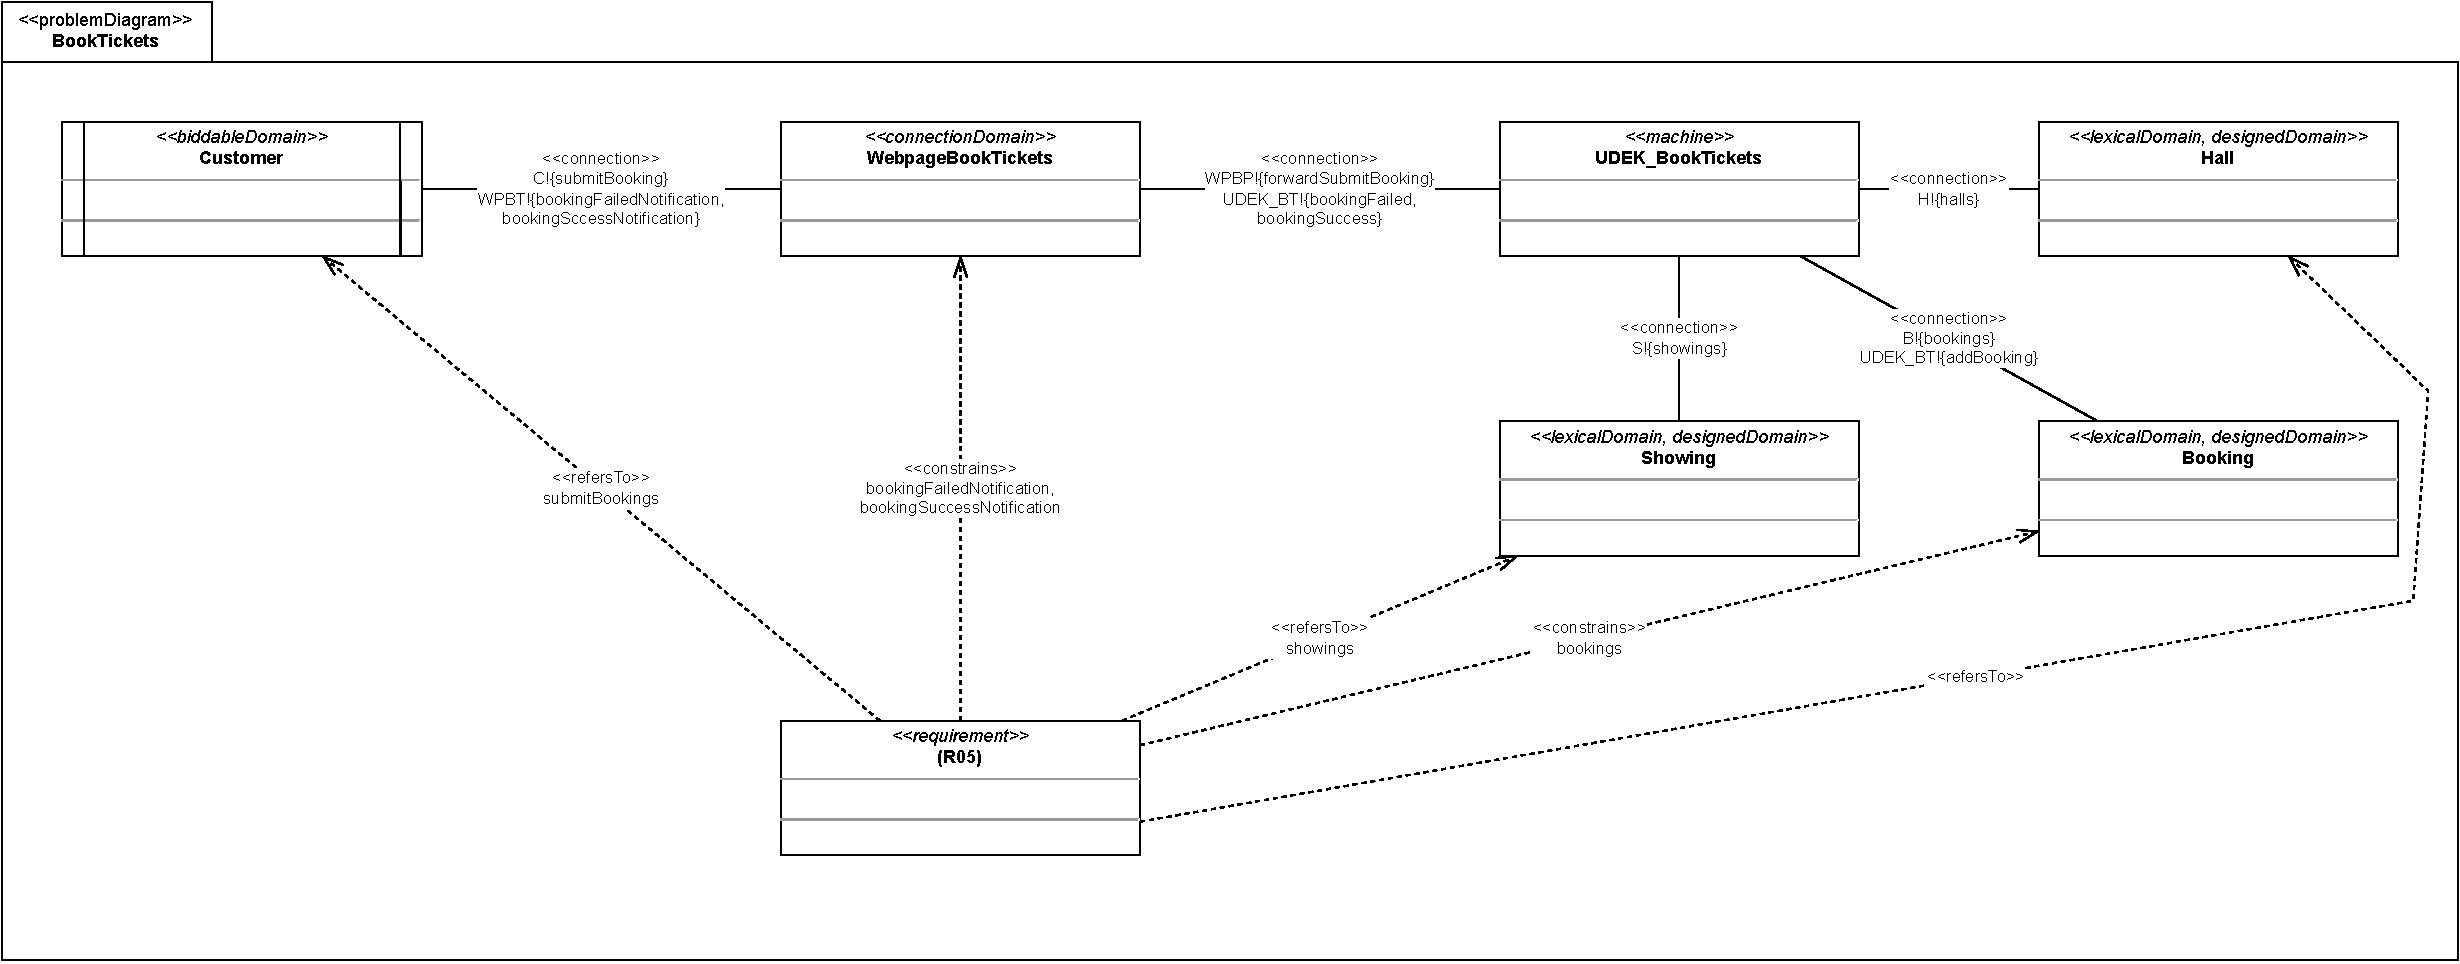
\includegraphics[width=0.9\textwidth]{figures/03/a03_problem_diagram_3-PD.pdf}
    \caption{Problem diagram for R\ref{enum:R5}}
    \label{figure:pdR5}
\end{figure}

\begin{figure}[H]
    \centering
    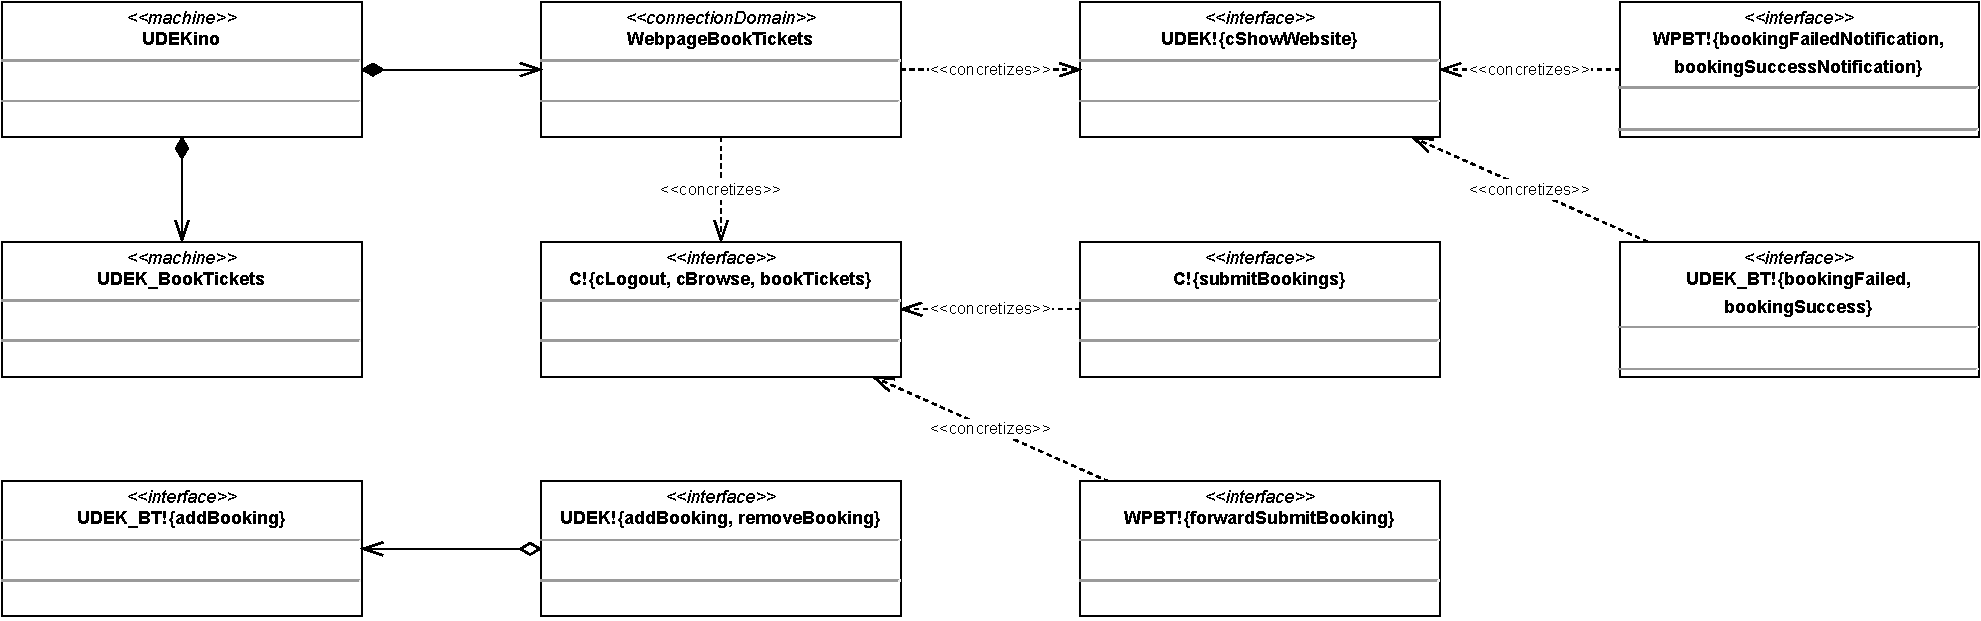
\includegraphics[width=0.9\textwidth]{figures/03/a03_problem_diagram_3-Mapping.pdf}
    \caption{Mapping diagram for R\ref{enum:R5}}
    \label{figure:mdR5}
\end{figure}

\begin{figure}[H]
\centering
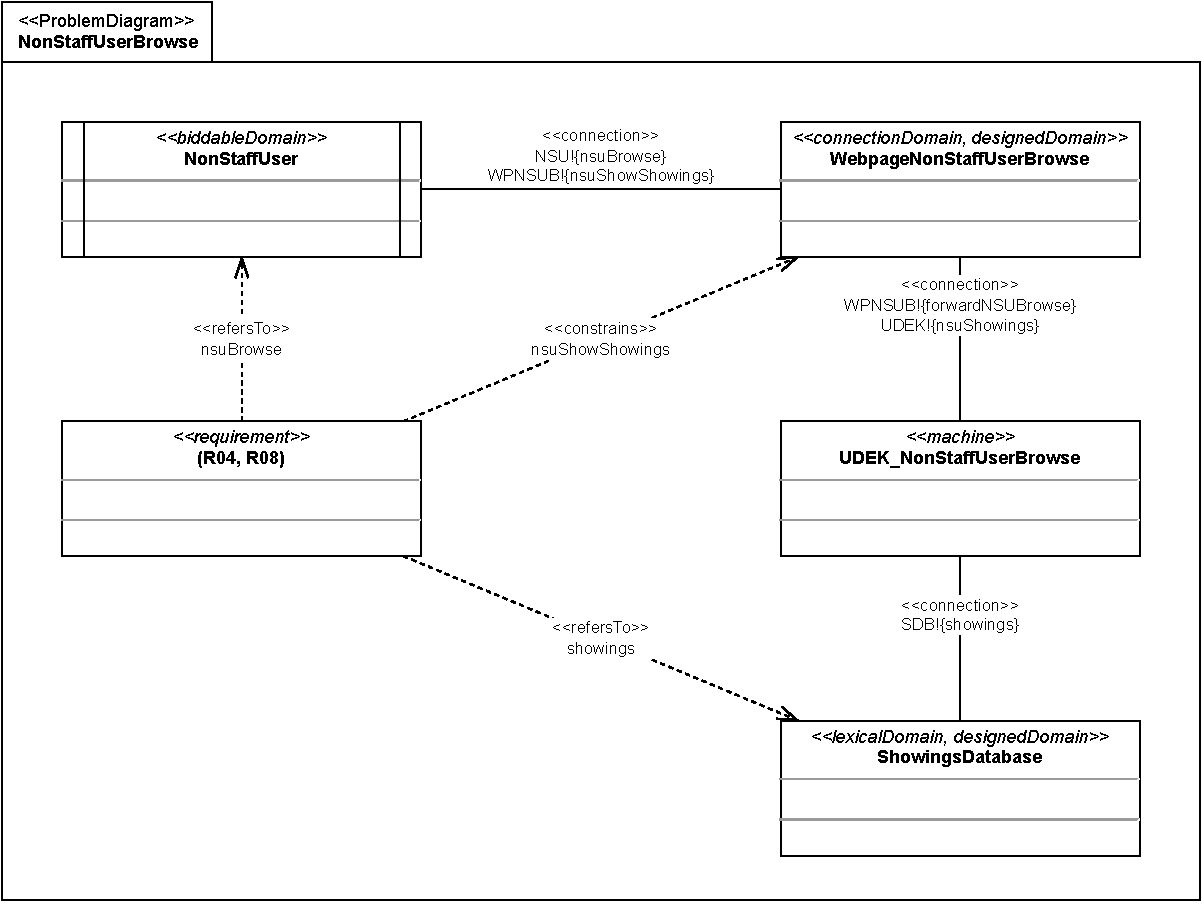
\includegraphics[width=0.9\textwidth]{figures/04/a04_problem_diagram_2-PD.pdf}
\caption{Problem diagram for R\ref{enum:R4} / R\ref{enum:R8}}
\label{figure:pdR48}
\end{figure}

\begin{figure}[H]
\centering
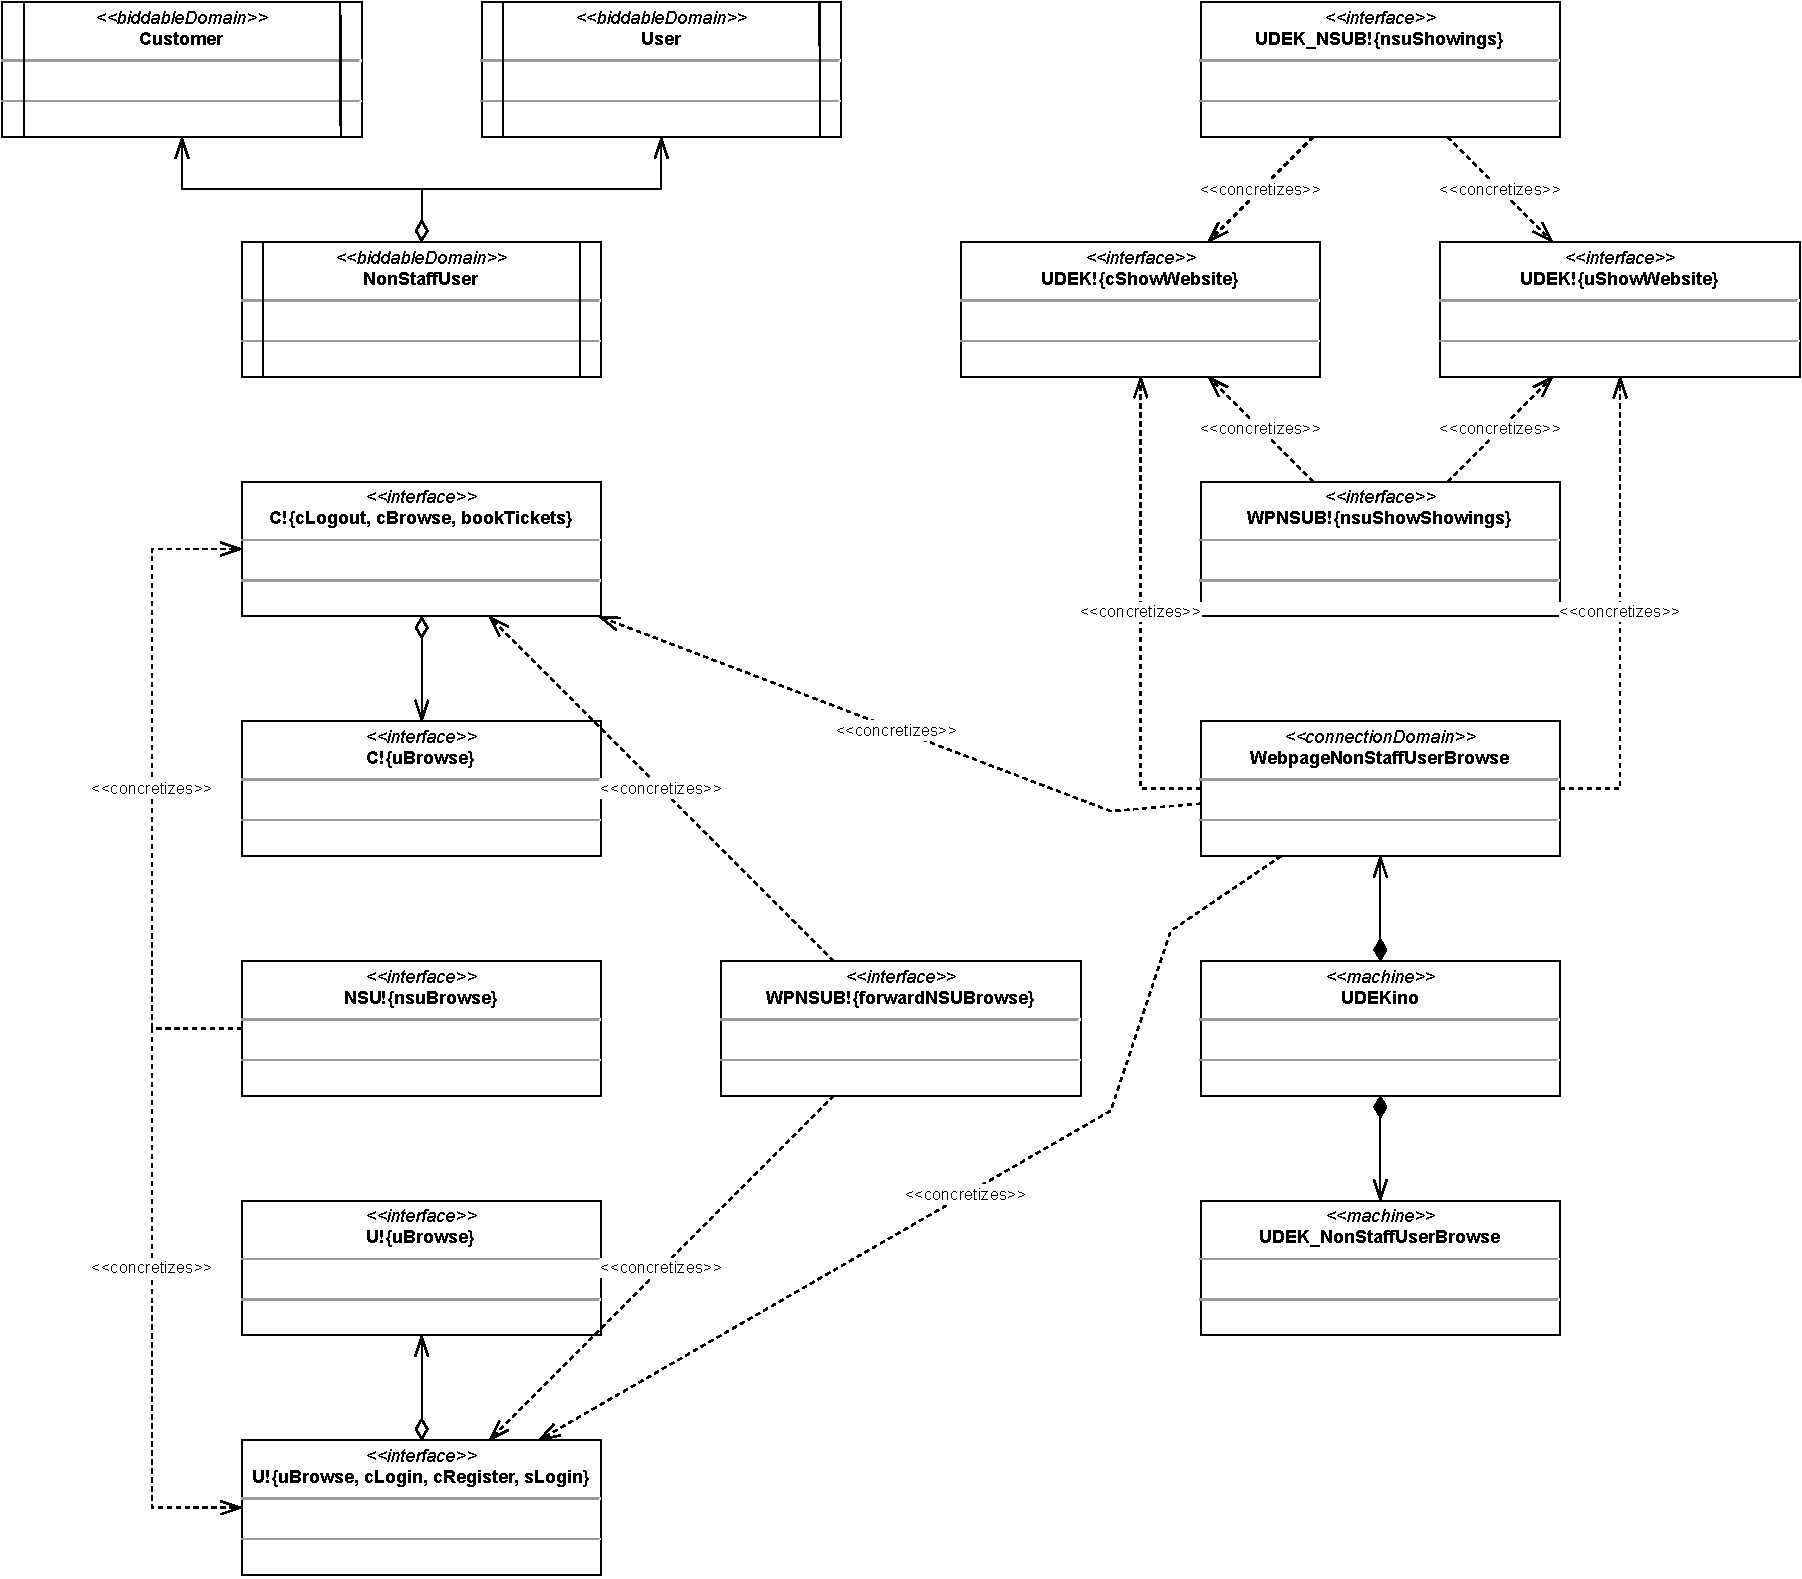
\includegraphics[width=0.9\textwidth]{figures/04/a04_problem_diagram_2-Mapping.pdf}
\caption{Mapping diagram for R\ref{enum:R4} / R\ref{enum:R8}}
\label{figure:mdR48}
\end{figure}

\begin{figure}[H]
\centering
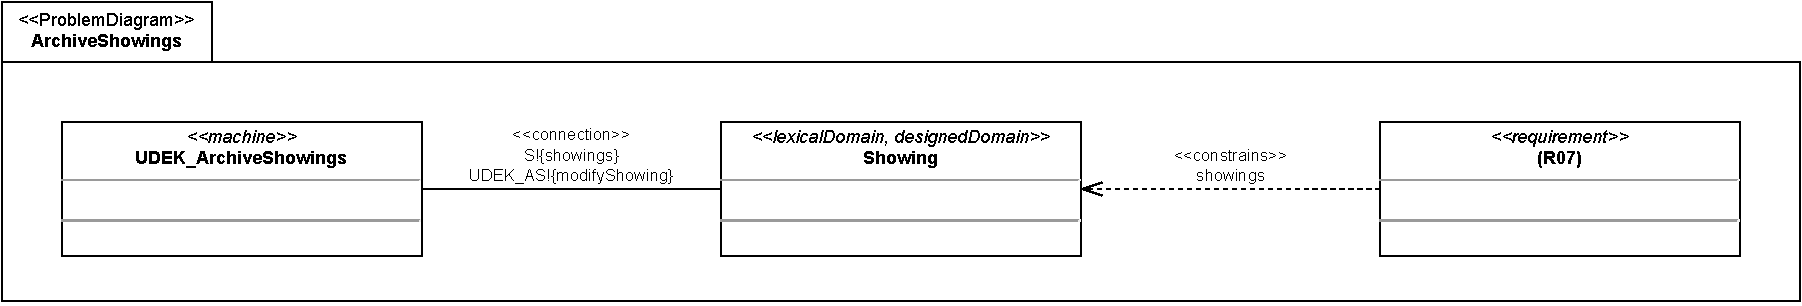
\includegraphics[width=0.9\textwidth]{figures/04/a04_problem_diagram_4-PD.pdf}
\caption{Problem diagram for R\ref{enum:R7}}
\label{figure:pdR7}
\end{figure}

\begin{figure}[H]
\centering
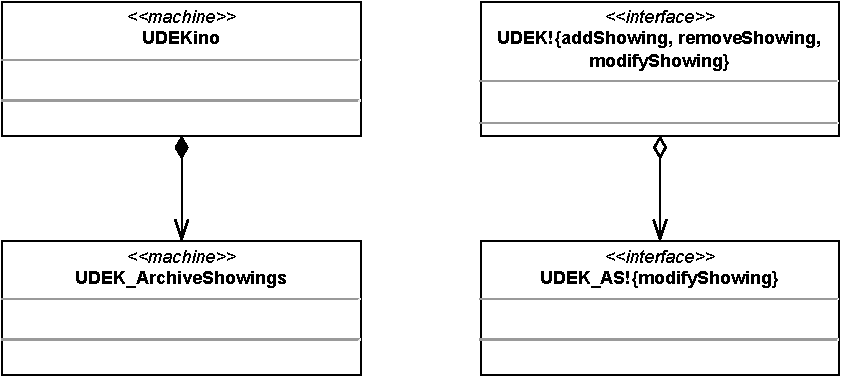
\includegraphics[width=0.9\textwidth]{figures/04/a04_problem_diagram_4-Mapping.pdf}
\caption{Mapping diagram for R\ref{enum:R7}}
\label{figure:mdR7}
\end{figure}

\subsection*{Frames}
\begin{itemize}
    \item R\ref{enum:R1} fits to update 2
    \item R\ref{enum:R5} fits to update 2
    \item R\ref{enum:R4} / R\ref{enum:R8} fits to query 2
    \item R\ref{enum:R7} fits to simple transformation
\end{itemize}

\newpage\section{A3}

\begin{figure}[H]
    \centering
    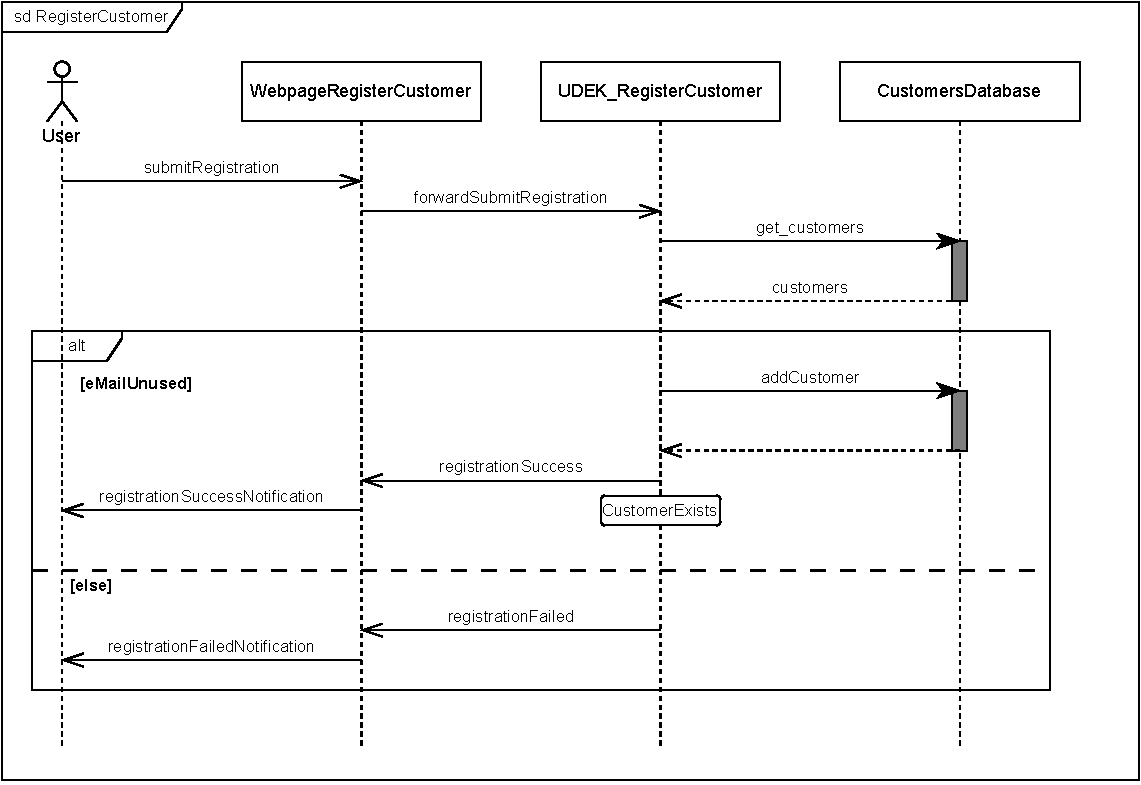
\includegraphics[width=0.9\textwidth]{figures/05/a05_sequence_diagram_r01.pdf}
    \caption{Sequence diagram for R\ref{enum:R1}}
    \label{figure:sdR1}
\end{figure}

\begin{itemize}
    \item[S1a] \textbf{WebpageRegisterCustomer}\\
    When the WebpageRegisterCustomer recieves the command "submitRegistration", the command is forwarded to machine with "forwardSubmitRegistration".
    Results are recieved via commands "registrationFailed" or "registrationSuccess" and displayed to the User via "registrationFailedNotification" / "registrationSuccessNotification".

    \item[S1b] \textbf{UDEK\_RegisterCustomer}\\
    When the machine receives the command ``fowardSubmitRegistration'' the availability of the e-mail address is checked against existing Customer accounts in the CustomersDatabase via ``get\_customers''.
    If the e-mail address is available, a new Customer account is created with the data from the forwarded request and added to the CustomersDatabase via ``addCustomers'' and a confirmation is sent to the WebpageRegisterCustomer via ``registrationSuccess''.
    If the e-mail address is not available, account creation fails and a failure notification is sent to the WebpageRegisterCustomer via ``registrationFailed''.

    \item[S1c] \textbf{CustomersDatabase}\\
    When the database receives the command ``get\_customers'', all Customer accounts are returned as the data ``customers''.
    When the database receives the command ``addCustomer'', the Customer account is added.
\end{itemize}

$(A2) \land (S1a) \land (S1b) \land (S1c) \implies (R\ref{enum:R1})$

\begin{figure}[H]
\centering
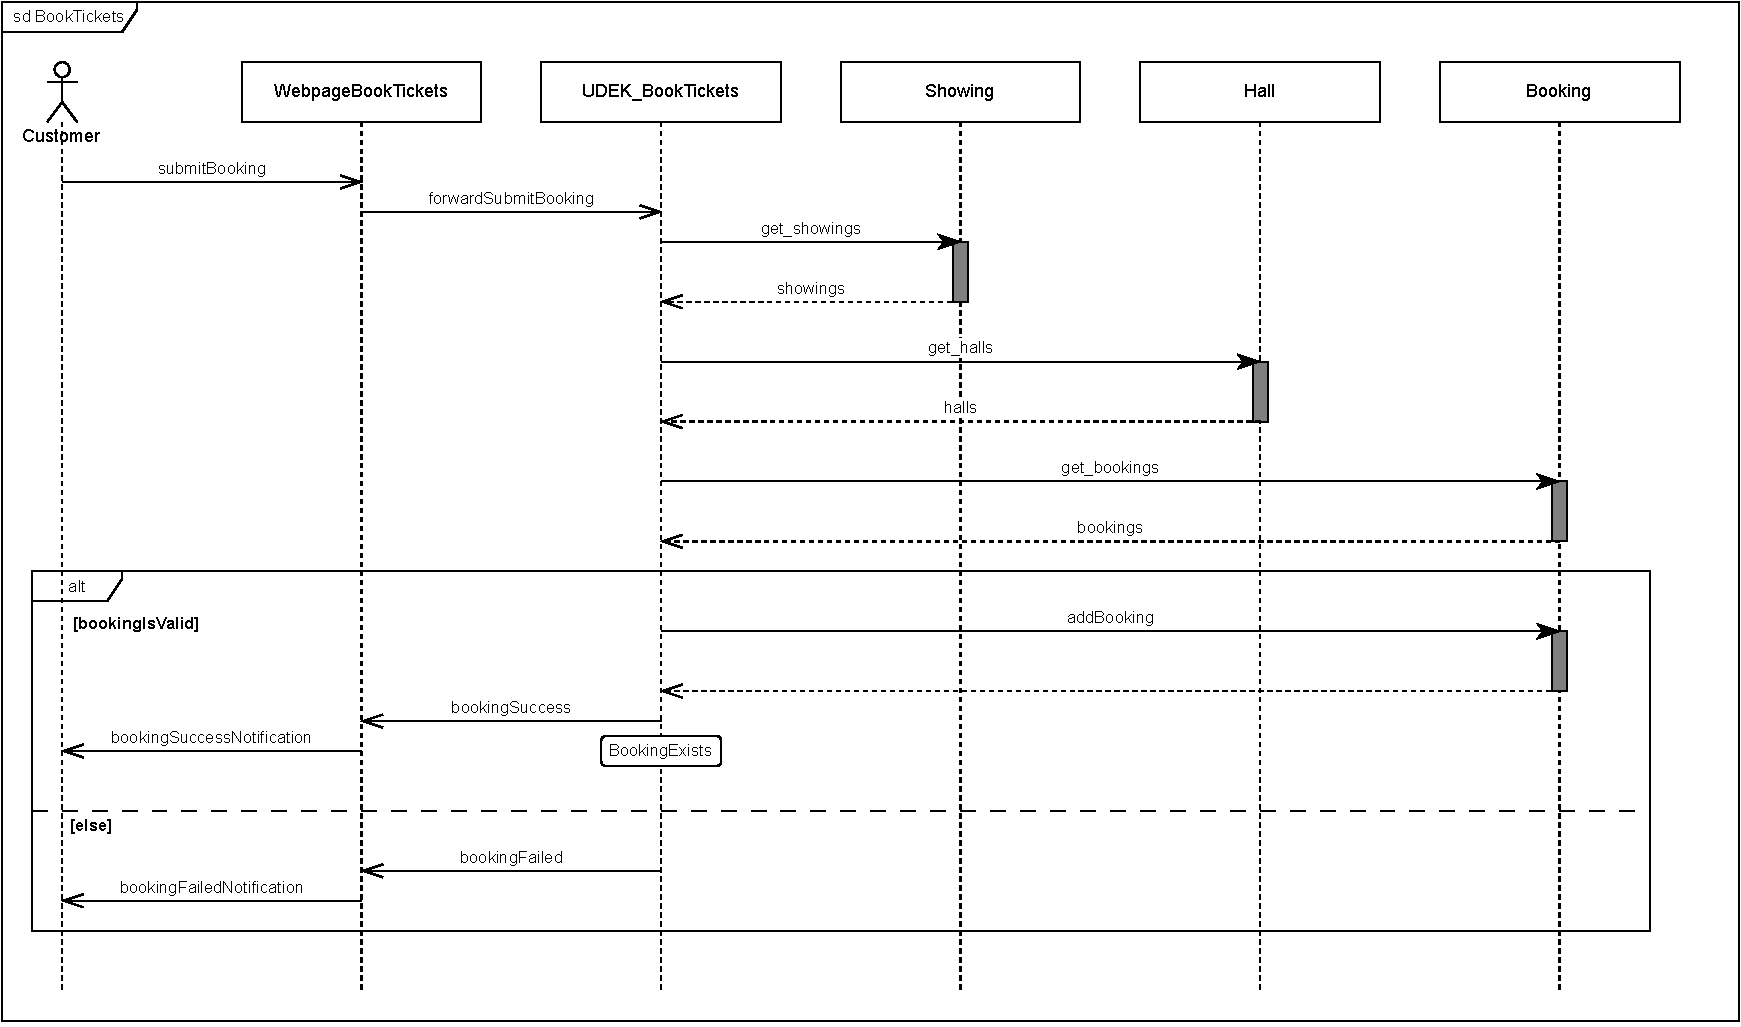
\includegraphics[width=0.9\textwidth]{figures/05/a05_sequence_diagram_r05.pdf}
\caption{Sequence diagram for R\ref{enum:R5}}
\label{figure:sdR5}
\end{figure}

\begin{itemize}
\item[S2a] \textbf{WebpageBookTickets}\\
When the Webpage receives the command ``submitBooking'', the command is forwarded to the machine with the command ``forwardSubmitBooking''.
Results are received via ``bookingFailed'' or ``bookingSuccess'' and displayed the the Customer via
``bookingFailedNotification'' / ``bookingSuccessNotification''

\item[S2b] \textbf{UDEK\_BookTickets}
When the machine receives the command ``forwardSubmitBooking'', the machine checks the availability of the desired showing and seats against the ShowingsDatabase, HallsDatabase and BookingsDatabase via ``get\_showings'', ``get\_halls'' and ``get\_bookings''.
If the desired showing and seats exist, the showing begins in more than 15 minutes and the seats are not already booked, the booking is added to the BookingsDatabase via ``addBooking'' and a success notification is sent to the WebpageBookTickets via ``bookingSuccess''.
Otherwise the booking fails and the Webpage is notified of the failure via ``bookingFailed''.

\item[S2c] \textbf{ShowingsDatabase}
When the database receives the command ``get\_showings'', all showings are returned as the data ``showings''.

\item[S2d] \textbf{HallsDatabase}
When the database receives the command ``get\_halls'', all halls are returned as the data ``halls''.

\item[S2c] \textbf{BookingsDatabase}
When the database receives the command ``get\_bookings'', all bookings are returned as the data ``bookings''.
When the database receives the command ``addBooking'', the booking is added.

\end{itemize}

$(F3) \land (S2a) \land (S2b) \land (S2c) \land (S2d) \land (S2e) \implies (R\ref{enum:R5})$

\begin{figure}[H]
    \centering
    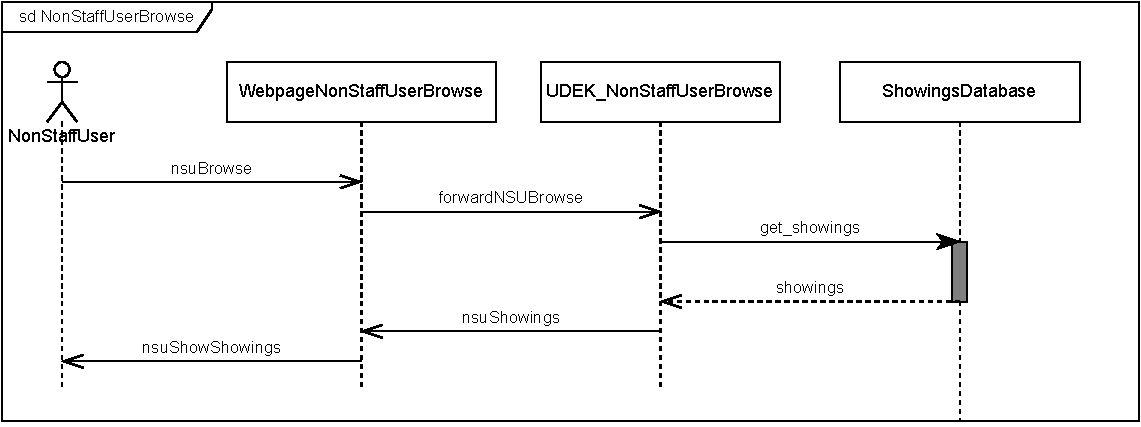
\includegraphics[width=0.9\textwidth]{figures/05/a05_sequence_diagram_r04r08.pdf}
    \caption{Sequence diagram for R\ref{enum:R4}/R\ref{enum:R8}}
    \label{figure:sdR48}
\end{figure}

\begin{itemize}
\item[S3a] \textbf{WebpageNonStaffUserBrowse}
When the Webpage receives the command ``nsuBrowse'', the command is forwarded to the machine with the command ``forwardNSUBrowse''.
Results are received via ``nsuShowings'' and displayed to NonStaffUser via ``nsuShowShowings''.

\item[S3b] \textbf{UDEK\_NonStaffUserBrowse}
When the machine receives the command "forwardNSUBrowse", the machine gets all showings from the ShowingsDatabase via ``get\_showings''.
All non-archived showings are send/transfered to the Webpage via ``nsuShowings''.

\item[S3c] \textbf{ShowingsDatabase}
When the database receives the command ``get\_showings'', all showings are returned data as ``showings''

\end{itemize}

$(S3a) \land (S3b) \land (S3c) \implies (R\ref{enum:R4}) \land (R\ref{enum:R8})$

\begin{figure}[H]
\centering
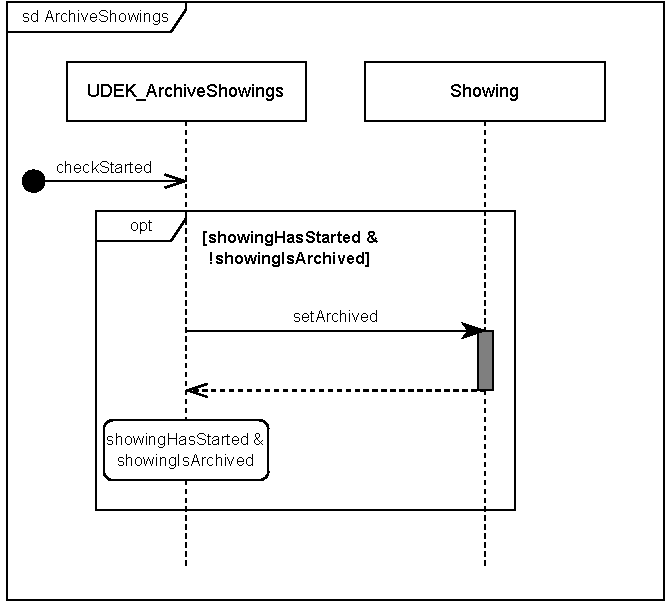
\includegraphics{figures/05/a05_sequence_diagram_r07.pdf}
\caption{Sequence diagram for R\ref{enum:R7}}
\label{figure:sdR7}
\end{figure}

\begin{itemize}
\item[S4a] \textbf{UDEK\_ArchiveShowings}
When receiving the command ``checkStarted'', all showings which have already started, and are not yet marked as archived, are marked as archived using the command ``setArchived''.

\item[S4b] \textbf{ShowingsDatabase}
When receiving the command ``setArchived'', all showings which have already started, and are not yet marked as archived, are marked as archived.

\end{itemize}

$(S4a) \land (S4b) \implies (R\ref{enum:R7})$

\newpage\section{A4}

\newpage\section{A5}
A short OCL example:\\
%-------------------
%-------------------The following used package provides an easy OCL syntax highlighting.
%-------------------You do not have to add linebreaks. It is done automatically.
%-------------------
\lstset{language=OCL}          % Set your language (you can change the language for each code-block optionally)

\begin{lstlisting}[frame=single,breaklines=true,numbers=left,numberfirstline=true]
context Person inv: self.alter >=0

pre alter>30
post alter=alter@pre+1

\end{lstlisting}

\newpage\section{A6}

Examples of a life-cycle using the math-environment:

$LC_{guest}=(Browse^+;[Book])^*$



\chapter{Design}

\section{D1}

\section{D2}

\section{D3}

\section{D4}

State diagrams with tikZ:
%Do not change, only declaration of the element
\tikzstyle{startpoint} = [circle, minimum width=0.5cm, minimum height=0.5cm, text centered, draw=black, fill=black]
\tikzstyle{endpoint} = [circle, minimum width=0.5cm, minimum height=0.5cm, text centered, draw=black, fill=white]
\tikzstyle{endin} = [circle, minimum width=0.05cm, minimum height=0.05cm, text centered, draw=black, fill=black]
\tikzstyle{state} = [rectangle, rounded corners, minimum width=2cm, minimum height=1cm, text centered, draw=black]
\tikzstyle{decision} = [diamond, minimum width=0.5cm, minimum height=0.5cm, text centered, draw=black]
\tikzstyle{arrow} = [->,>=stealth]
\tikzstyle{every node} = [font=\tiny]

%--------------
%--------------We use the same figure environment as for pictures to reference diagrams with tikz.
%--------------Here we provide a small example how to draw a state machine with tikZ.
%--------------The picture is created only with this commands.
%--------------
\begin{figure}[H]
\caption{Zustandsdiagramm Person 1}
\label{d1:zustand1}
\begin{tikzpicture}[node distance=2cm]

%Knoten
\node (Start) [startpoint]{};
\node (State1) [state, right= of Start] {State 1};
\draw [arrow] (Start) -- (State1);

\node (Decision1) [decision, right= of State1]{};
\draw [arrow] (State1) -- (Decision1)  node [pos=0.5,below,fill=white] {Annotation};

\node (State2) [state, below= of Decision1] {State 2};
\draw [arrow] (Decision1) -- (State2)  node [pos=0.2,below,fill=white] {true};



\node (End) [endpoint,right= of State2]{\begin{tikzpicture}\node (End) [endin]{};\end{tikzpicture}};
\draw [arrow] (State2) -- (End);
\draw [arrow] (Decision1) -| (End)  node [pos=0.2,left,fill=white] {false};
\end{tikzpicture}
\end{figure}



\chapter{Implementation \& Testing}

%---------------
%---------------You do not have to copy your source code.
%---------------Just use the given space to add any comments or explanations.
%---------------

\section{I}

\section{T1}

\section{T2}

\section{T3}




%-------------------------
%-------------------------
%--------The glossary makes use of the package longtable to allow automatic page breaks
%-------------------------
%-------------------------
\chapter{Glossary}

\begin{longtable}{|l|p{3cm}|p{5cm}|l|}
\caption{Glossary}
\label{table:glossar}\\
\hline
\rowcolor{black!25}\textbf{Name} & \textbf{Type} & \textbf{Description} & \textbf{Source}\\
\hline
\endfirsthead
\caption[]{Glossary}\\
\hline
\rowcolor{black!25}\textbf{Name} & \textbf{Type} & \textbf{Description} & \textbf{Source}\\
\endhead
\hline
\endfoot
\multicolumn{4}{|l|}{\textbf{A}}\\
\hline
\hypertarget{glossary:addBooking}{addBooking} & phenomenon & the \hyperlink{glossary:UDEKino}{machine} adds a new booking to the \hyperlink{glossary:BookingsDatabase}{bookings database} & CD\\
\hline
addBooking & message & contains a showing ID and seats & SD R5\\
\hline
\hypertarget{glossary:addCustomer}{addCustomer} & phenomenon & the \hyperlink{glossary:UDEKino}{machine} adds a new \hyperlink{glossary:Customer}{customer} to the \hyperlink{glossary:CustomersDatabase}{customers database} & CD\\
\hline
addCustomer & message & contains an e-mail address and a password & SD R\ref{enum:R1}\\
\hline
\hypertarget{glossary:addShowing}{addShowing} & phenomenon & the \hyperlink{glossary:UDEKino}{machine} adds a new showing to the \hyperlink{glossary:ShowingsDatabase}{customers database} & CD\\
\hline
%-------------------------
%-------------------------
%--------Each element of the table is expressed in the following way:
%--------Cells are divided by & and each row ends with \\ (linebreak).
%--------The line between two rows is added with \hline.
%-------------------------
%-------------------------
%-------------------------
%-------------------------
\multicolumn{4}{|l|}{\textbf{B}}\\
\hline
BookingExists & state predicate & given booking exists within the BookingsDatabase & SD R5\\
\hline
\hypertarget{glossary:bookingFailed}{bookingFailed} & phenomenon & \hyperlink{glossary:UDEKino}{the machine} notifies \hyperlink{glossary:WebpageBookTickets}{the webpage} that a booking has failed & PD R\ref{enum:R5}\\
\hline
bookingFailed & message & informs the WebpageBookTickets that the booking failed & SD R5\\
\hline
\hypertarget{glossary:bookingFailedNotification}{bookingFailedNotification} & phenomenon & \hyperlink{glossary:WebpageBookTickets}{the webpage} displays a notification to \hyperlink{glossary:Customer}{the customer} that a booking has failed & PD R\ref{enum:R5}\\
\hline
bookingFailedNotification & message & informs the user that the booking failed & SD R5\\
\hline
bookingIsValid & guard & showing with ID contained in request exists and starts in more than 15 minutes and the seats contained in the request exist in the showing's hall and are not already booked & SD R5\\
\hline
bookings & message & all bookings in the BookingsDatabase & PD R5\\
\hline
\hypertarget{glossary:bookingSuccess}{bookingSuccess} & phenomenon & \hyperlink{glossary:UDEKino}{the machine} notifies \hyperlink{glossary:WebpageBookTickets}{the webpage} that a booking has succeeded & PD R\ref{enum:R5}\\
\hline
bookingSuccess & message & informs the WebpageBookTickets that the booking was successful & SD R5\\
\hline
\hypertarget{glossary:bookingSuccessNotification}{bookingSuccessNotification} & phenomenon & \hyperlink{glossary:WebpageBookTickets}{the webpage} displays a notification to \hyperlink{glossary:Customer}{the customer} that a booking has succeeded & PD R\ref{enum:R5}\\
\hline
bookingSuccessNotification & message & informs the Customer that the booking was successful & SD R5\\
\hline
\hypertarget{glossary:BookingsDatabase}{BookingsDatabase} & lexical domain, designed domain & a database containing the bookings made by \hyperlink{glossary:Customer}{customers} & CD\\
\hline
BookingsDatabase & object & the database containing all bookings & SD R5\\
\hline
\hypertarget{glossary:bookTickets}{bookTickets} & phenomenon & a \hyperlink{glossary:Customer}{customer} books tickets for a showing & CD\\
\hline
\multicolumn{4}{|l|}{\textbf{C}}\\
\hline
\hypertarget{glossary:cBrowse}{cBrowse} & phenomenon & a \hyperlink{glossary:Customer}{customer} browses available showings & CD\\
\hline
checkStarted & found message & a prompt for the UDEK\_ArchiveShowings machine to mark all showings which have already started and are not marked as archived, as archived & SD R7\\
\hline
\hypertarget{glossary:cLogin}{cLogin} & phenomenon & a \hyperlink{glossary:User}{user} attempts to log into a \hyperlink{glossary:Customer}{customer} account & CD\\
\hline
\hypertarget{glossary:cLogout}{cLogout} & phenomenon & a \hyperlink{glossary:Customer}{customer} attempts to log out & CD\\
\hline
\hypertarget{glossary:cRegister}{cRegister} & phenomenon & a \hyperlink{glossary:User}{user} attempts to create customer account on UDEKino & CD\\
\hline
\hypertarget{glossary:cShowWebsite}{cShowWebsite} & phenomenon & the \hyperlink{glossary:UDEKino}{machine} shows a website to the \hyperlink{glossary:Customer}{customer} & CD\\
\hline
\hypertarget{glossary:Customer}{Customer} & biddable domain & a customer of UDEKino; a \hyperlink{glossary:User}{user} who has logged into a customer account & CD\\
\hline
Customer & actor & a customer who wishes to book tickets & SD R5\\
\hline
CustomerExists & state predicate & the customer account with the given e-mail address and password exists within the CustomersDatabase & SD R\ref{enum:R1}\\
\hline
customers & message & all customers in the CustomersDatabase & SD R\ref{enum:R1}\\
\hline
\hypertarget{glossary:CustomersDatabase}{CustomersDatabase} & lexical domain, designed domain & a database containing \hyperlink{glossary:Customer}{customer} data & CD\\
\hline
CustomersDatabase & object & the database of customer acccounts & SD R\ref{enum:R1}\\
\hline
\multicolumn{4}{|l|}{\textbf{D}}\\
\hline
\hypertarget{glossary:displayNotification}{displayNotification} & phenomenon & the \hyperlink{glossary:Customer}{customer's} \hyperlink{glossary:Email}{e-mail client} displays a \hyperlink{glossary:notifyCustomer}{notification e-mail} to the \hyperlink{glossary:Customer}{customer} & CD\\
\hline
\multicolumn{4}{|l|}{\textbf{E}}\\
\hline
\hypertarget{glossary:Email}{Email} & causal domain, connection domain & an e-mail service offering to deliver e-mails & CD\\
\hline
eMailAvailable & guard & the e-mail contained in the registration request is not contained in customers & SD R\ref{enum:R1}\\
\hline
\multicolumn{4}{|l|}{\textbf{F}}\\
\hline
\hline
\hypertarget{glossary:forwardNSUBrowse}{forwardNSUBrowse} & phenomenon & \hyperlink{glossary:WebPageNonStaffUserBrowse}{the website} sends a request for a list of upcoming showings to \hyperlink{glossary:UDEK-NonStaffUserBrowse}{the machine} & PD R\ref{enum:R4} / R\ref{enum:R8}\\
\hline
forwardNSUBrowse & message & a request for the machine to send a list of available, i.e., non-archived, showings & SD R4/8\\
\hline
\hypertarget{glossary:forwardSubmitBooking}{forwardSubmitBooking} & phenomenon & \hyperlink{glossary:WebpageBookTickets}{the webpage} forwards a request to book tickets to \hyperlink{glossary:UDEKino}{the machine} & PD R\ref{enum:R5}\\
\hline
forwardSubmitBooking & message & contains the showing ID and the desired seats & SD R5\\
\hline
\hypertarget{glossary:forwardSubmitRegistration}{forwardSubmitRegistration} & phenomenon & \hyperlink{glossary:WebpageRegisterCustomer}{the webpage} forwards a request to register a \hyperlink{glossary:Customer}{customer account} to \hyperlink{glossary:UDEKino}{the machine} & PD R\ref{enum:R1}\\
\hline
forwardSubmitRegistration & message & a request from the WebpageRegisterCustomer to register a new customer account, containing an e-mail address and a password & SD R\ref{enum:R1}\\
\hline
\multicolumn{4}{|l|}{\textbf{G}}\\
\hline
get\_bookings & message & contains all messages in the BookingsDatabase & SD R5\\
\hline
get\_customers & message & returns all customer accounts in the CustomersDatabase & SD R\ref{enum:R1}\\
\hline
get\_halls & message & returns all halls in the HallsDatabase & SD R5\\
\hline
get\_showings & message & returns all showings in the ShowingsDatabase & SD R5, 4/8, 7\\
\hline
\multicolumn{4}{|l|}{\textbf{H}}\\
\hline
halls & message & all halls in the HallsDatabase & SD R5\\
\hline
\hypertarget{glossary:HallsDatabase}{HallsDatabase} & lexical domain & a database containing the cinema halls, provided by the cinema operator & CD\\
\hline
HallsDatabase & object & the database containing the cinema halls & SD R5\\
\hline
\multicolumn{4}{|l|}{\textbf{I}}\\
\hline
&  &  & \\
\hline
\multicolumn{4}{|l|}{\textbf{J}}\\
\hline
&  &  & \\
\hline
\multicolumn{4}{|l|}{\textbf{K}}\\
\hline
&  &  & \\
\hline
\multicolumn{4}{|l|}{\textbf{L}}\\
&  &  & \\
\hline
\multicolumn{4}{|l|}{\textbf{M}}\\
\hline
\hypertarget{glossary:modifyShowing}{modifyShowing} & phenomenon & \hyperlink{glossary:UDEKino}{the machine} modifies a showing in the \hyperlink{glossary:ShowingsDatabase}{showings database} & CD\\
\hline
\multicolumn{4}{|l|}{\textbf{N}}\\
\hline
\hypertarget{glossary:NonStaffUser}{NonStaffUser} & biddable domain & either of \hyperlink{glossary:Customer}{Customer} or \hyperlink{glossary:User}{User} & PD R\ref{enum:R4} / R\ref{enum:R8}\\
\hline
NonStaffUser & actor & a user who is not logged in as staff and wishes to browse available showings & SD R4/8\\
\hline
\hypertarget{glossary:notifyCustomer}{notifyCustomer} & phenomenon & the \hyperlink{glossary:UDEKino}{machine} notifies the \hyperlink{glossary:Customer}{customer} via \hyperlink{glossary:Email}{e-mail} & CD\\
\hline
\hypertarget{glossary:nsuBrowse}{nsuBrowse} & phenomenon & either of \hyperlink{glossary:cBrowse}{cBrowse} or \hyperlink{glossary:uBrowse}{uBrowse} & PD R\ref{enum:R4} / R\ref{enum:R8}\\
\hline
nsuBrowse & message & a request for the WebpageNonStaffUserBrowse to display available showings & SD R4/8\\
\hline
\hypertarget{glossary:nsuShowings}{nsuShowings} & phenomenon & \hyperlink{glossary:UDEK-NonStaffUserBrowse}{the machine} sends a list of upcoming showings to be displayed by \hyperlink{glossary:WebPageNonStaffUserBrowse}{the website} & PD R\ref{enum:R4} / R\ref{enum:R8}\\
\hline
nsuShowings & message & contains available, i.e., non-archived, showings & SD R4/8\\
\hline
\hypertarget{glossary:nsuShowShowings}{nsuShowShowings} & phenomenon & \hyperlink{glossary:WebPageNonStaffUserBrowse}{the website} displays a list of upcoming showings to the \hyperlink{glossary:NonStaffUser}{user} & PD R\ref{enum:R4} / R\ref{enum:R8}\\
\hline
nsuShowShowings & message & a rendition of available, i.e., non-archived, showings & SD R4/8\\
\hline
\multicolumn{4}{|l|}{\textbf{O}}\\
\hline
&  &  & \\
\hline
\multicolumn{4}{|l|}{\textbf{P}}\\
\hline
\hypertarget{glossary:bookings}{bookings} & phenomenon & the \hyperlink{glossary:BookingsDatabase}{bookings database} provides the bookings data to the \hyperlink{glossary:UDEKino}{machine} & CD\\
\hline
\hypertarget{glossary:customers}{customers} & phenomenon & the \hyperlink{glossary:CustomersDatabase}{customers database} provides the customers data to the \hyperlink{glossary:UDEKino}{machine} & CD\\
\hline
\hypertarget{glossary:halls}{halls} & phenomenon & the \hyperlink{glossary:HallsDatabase}{halls database} provides the halls data to the \hyperlink{glossary:UDEKino}{machine} & CD\\
\hline
\hypertarget{glossary:showings}{showings} & phenomenon & the \hyperlink{glossary:ShowingsDatabase}{showings database} provides the showings data to the \hyperlink{glossary:UDEKino}{machine} & CD\\
\hline
\multicolumn{4}{|l|}{\textbf{Q}}\\
\hline
&  &  & \\
\hline
\multicolumn{4}{|l|}{\textbf{R}}\\
\hline
\hypertarget{glossary:registrationFailed}{registrationFailed} & phenomenon & \hyperlink{glossary:UDEKino}{the machine} notifies \hyperlink{glossary:WebpageRegisterCustomer}{the webpage} that the registration has failed & PD R\ref{enum:R1}\\
\hline
registrationFailed & message & informs the WebpageRegisterCustomer that account creation has failed & SD R\ref{enum:R1}\\
\hline
\hypertarget{glossary:registrationFailedNotification}{registrationFailedNotification} & phenomenon & \hyperlink{glossary:WebpageRegisterCustomer}{the webpage} displays a to \hyperlink{glossary:User}{the user} that the registration has failed & PD R\ref{enum:R1}\\
\hline
registrationFailedNotification & message & informs the user that account creation has succeeded & SD R\ref{enum:R1}\\
\hline
\hypertarget{glossary:registrationSuccess}{registrationSuccess} & phenomenon & \hyperlink{glossary:UDEKino}{the machine} notifies \hyperlink{glossary:WebpageRegisterCustomer}{the webpage} that the registration has succeeded & PD R\ref{enum:R1}\\
\hline
registrationSuccess & message & informs the WebpageRegisterCustomer that account registration has succeeded & SD R\ref{enum:R1}\\
\hline
\hypertarget{glossary:registrationSuccessNotification}{registrationSuccessNotification} & phenomenon & \hyperlink{glossary:WebpageRegisterCustomer}{the webpage} displays a notification to \hyperlink{glossary:User}{the user} that the registration has succeeded & PD R\ref{enum:R1}\\
\hline
registrationSuccessNotification & message & informs the User that account creation has succeeded & SD R\ref{enum:R1}\\
\hline
\hypertarget{glossary:removeBooking}{removeBooking} & phenomenon &  \hyperlink{glossary:UDEKino}{the machine} removes a booking from the \hyperlink{glossary:BookingsDatabase}{bookings database} & CD\\
\hline
\hypertarget{glossary:removeBooking}{removeCustomer} & phenomenon &  \hyperlink{glossary:UDEKino}{the machine} removes a \hyperlink{glossary:Customer}{customer} from the \hyperlink{glossary:CustomersDatabase}{customers database} & CD\\
\hline
\hypertarget{glossary:Showing}{removeShowing} & phenomenon &  \hyperlink{glossary:UDEKino}{the machine} removes a showing from the \hyperlink{glossary:ShowingsDatabase}{showings database} & CD\\
\hline
\multicolumn{4}{|l|}{\textbf{S}}\\
\hline
\hypertarget{glossary:sBrowse}{sBrowse} & phenomenon & a \hyperlink{glossary:StaffMember}{staff member} browses available showings & CD\\
\hline
\hypertarget{glossary:sCancelShowing}{sCancelShowing} & phenomenon & a \hyperlink{glossary:StaffMember}{staff member} attempts to cancel a showing & CD\\
\hline
setArchived & message & contains the ID of the showing which is to be marked as archived & SD R7\\
\hline
ShowingHasStarted & guard / state predicate & whether the showing in question has already started, i.e., its starting date and time lies in the past & SD R7\\
\hline
ShowingIsArchived & guard / state predicate & whether the showing in question is marked as archived" & SD R7\\
\hline
showings & message & contains all showings in the ShowingsDatabase & SD R5, 4/8, 7\\
\hline
\hypertarget{glossary:ShowingsDatabase}{ShowingsDatabase} & lexical domain, designed domain & a database containing the cinema showings & CD\\
\hline
ShowingsDatabase & object & the database containing the showings & SD R5, 4/8, 7\\
\hline
\hypertarget{glossary:sLogin}{sLogin} & phenomenon & a \hyperlink{glossary:User}{user} attempts to log in as a \hyperlink{glossary:StaffMember}{staff member} & CD\\
\hline
\hypertarget{glossary:sLogout}{sLogout} & phenomenon & a \hyperlink{glossary:StaffMember}{staff member} attempts to log out & CD\\
\hline
\hypertarget{glossary:sShowWebsite}{sShowWebsite} & phenomenon & the \hyperlink{glossary:UDEKino}{machine} shows a website to the \hyperlink{glossary:StaffMember}{staff member} & CD\\
\hline
\hypertarget{glossary:StaffMember}{StaffMember} & biddable domain & a member of cinema staff; a \hyperlink{glossary:User}{user} who has logged in as staff & CD\\
\hline
\hypertarget{glossary:submitBooking}{submitBooking} & phenomenon & the \hyperlink{glossary:Customer}{customer} selects the tickets they wish to book and hits the submit button &  PD R\ref{enum:R5}\\
\hline
submitBookign & message & contains the showing ID and desired seats & SD R5\\
\hline
\hypertarget{glossary:submitRegistration}{submitRegistration} & phenomenon & the \hyperlink{glossary:User}{user} submits a request to register a new \hyperlink{glossary:Customer}{customer} account, containing an e-mail address and a password & PD R\ref{enum:R1}\\
\hline
\hline
submitRegistration & message & a request from the user to register a new customer account, containing an e-mail address and a password & SD R\ref{enum:R1}\\
\hline
\hypertarget{glossary:submitShowing}{submitShowing} & phenomenon & a \hyperlink{glossary:StaffMember}{staff member} submits a new showing to the machine for entry into the database & CD\\
\hline
\multicolumn{4}{|l|}{\textbf{T}}\\
\hline
&  &  & \\
\hline
\multicolumn{4}{|l|}{\textbf{U}}\\
\hline
\hypertarget{glossary:uBrowse}{uBrowse} & phenomenon & a \hyperlink{glossary:User}{user} browses available showings & CD\\
\hline
\hypertarget{glossary:UDEKino}{UDEKino} & machine & the machine to be developed & CD\\
\hline
\hypertarget{glossary:UDEK-ArchiveShowings}{UDEK\_ArchiveShowings} & machine & the sub-\hyperlink{glossary:UDEKino}{machine} responsible for automatically archiving showings once they have begun & PD R\ref{enum:R7} \\
\hline
UDEK\_ArchiveShowings & object & the sub-machine responsible for archiving showings which have already started & SD R7\\
\hline
\hypertarget{glossary:UDEK-BookTickets}{UDEK\_BookTickets} & machine & the sub-\hyperlink{glossary:UDEKino}{machine} responsible for \hyperlink{glossary:Customer}{customer} booking tickets & PD R\ref{enum:R5}\\
\hline
UDEK\_BookTickets & object & the machine responsible for the booking of tickets & SD R5\\
\hline
\hypertarget{glossary:UDEK-NonStaffUserBrowse}{UDEK\_NonStaffUserBrowse} & machine & the sub-\hyperlink{glossary:UDEKino}{machine} responsible for \hyperlink{glossary:NonStaffUser}{registered and non-registered} customers browsing upcoming showings & PD R\ref{enum:R4} / R\ref{enum:R8}\\
\hline
\hypertarget{glossary:UDEK-RegisterCustomer}{UDEK\_RegisterCustomer} & machine & the sub-\hyperlink{glossary:UDEKino}{machine} responsible for \hyperlink{glossary:Customer}{customer} account registration & PD R\ref{enum:R1}\\
\hline
UDEK\_RegisterCustomer & object & the machine responsible for customer account registration & SD R\ref{enum:R1}\\
\hline
\hypertarget{glossary:User}{User} & biddable domain & a user of the \hyperlink{glossary:UDEKino}{application} who is not logged in & CD\\
\hline
User & actor & a user of who wishes to register a new customer account & SD R\ref{R1}\\
\hline
\hypertarget{glossary:uShowWebsite}{uShowWebsite} & phenomenon & the \hyperlink{glossary:UDEKino}{machine} shows a website to the \hyperlink{glossary:User}{user} & CD\\
\hline
\multicolumn{4}{|l|}{\textbf{V}}\\
\hline
&  &  & \\
\hline
\multicolumn{4}{|l|}{\textbf{W}}\\
\hline
\hypertarget{glossary:WebpageBookTickets}{WebpageBookTickets} & connection domain, designed domain & a webpage via which a \hyperlink{glossary:Customer}{customer} can book tickets & PD R\ref{enum:R5}\\
\hline
WebpageBookTickets & object & the webpage for booking tickets & SD R5\\
\hline
\hypertarget{glossary:WebpageNonStaffUserBrowse}{WebpageNonStaffUserBrowse} & connection domain, designed domain & a webpage via which a \hyperlink{glossary:NonStaffUser}{user} can browse upcoming showings & PD R\ref{enum:R4} / R\ref{enum:R8}\\
\hline
WebpageNonStaffUserBrowse & object & the webpage for NonStaffUsers to browse available showings & SD R4/8\\
\hline
\hypertarget{glossary:WebpageRegisterCustomer}{WebpageRegisterCustomer} & connection domain, designed domain & a webpage via which a \hyperlink{glossary:User}{user} can register a new \hyperlink{glossary:Customer}{customer account} & PD R\ref{enum:R1}\\
\hline
WebpageRegisterCustomer & object & the webpage for registering a new customer account & SD R\ref{enum:R1}\\
\hline
\multicolumn{4}{|l|}{\textbf{X}}\\
\hline
&  &  & \\
\hline
\multicolumn{4}{|l|}{\textbf{Y}}\\
\hline
&  &  & \\
\hline
\multicolumn{4}{|l|}{\textbf{Z}}\\
\hline
&  &  & \\
\hline
\end{longtable}

\end{document}